%!TEX root = ../../thesis.tex

\graphicspath{{Chapters/appendix_bonsai/figures/}}
\chapter{BonsaiNet Architecture Diagrams and Supplementary Algorithms} \label{chapter:bonsai_architectures}
\section{Edges} \label{sect:bonsai_appendix_edges}
Edges (Figure~\ref{fig:bonsai_edge}) take some single input and pass it through $|\mathcal{O}|$ parallel operations.
The results of these operations are then individually pruned, and the edge outputs a list of these pruned operation outputs.
A critical distinction to make here is that these special Bonsai edges that perform this parallel operation pruning will
be represented in \color{red}red\color{black}, while normal graph edges are represented in black. These
normal graph edges simply indicate unmodified data flow between components of the model.
\begin{figure}[ht]
	\centering
	 \hspace*{-3cm}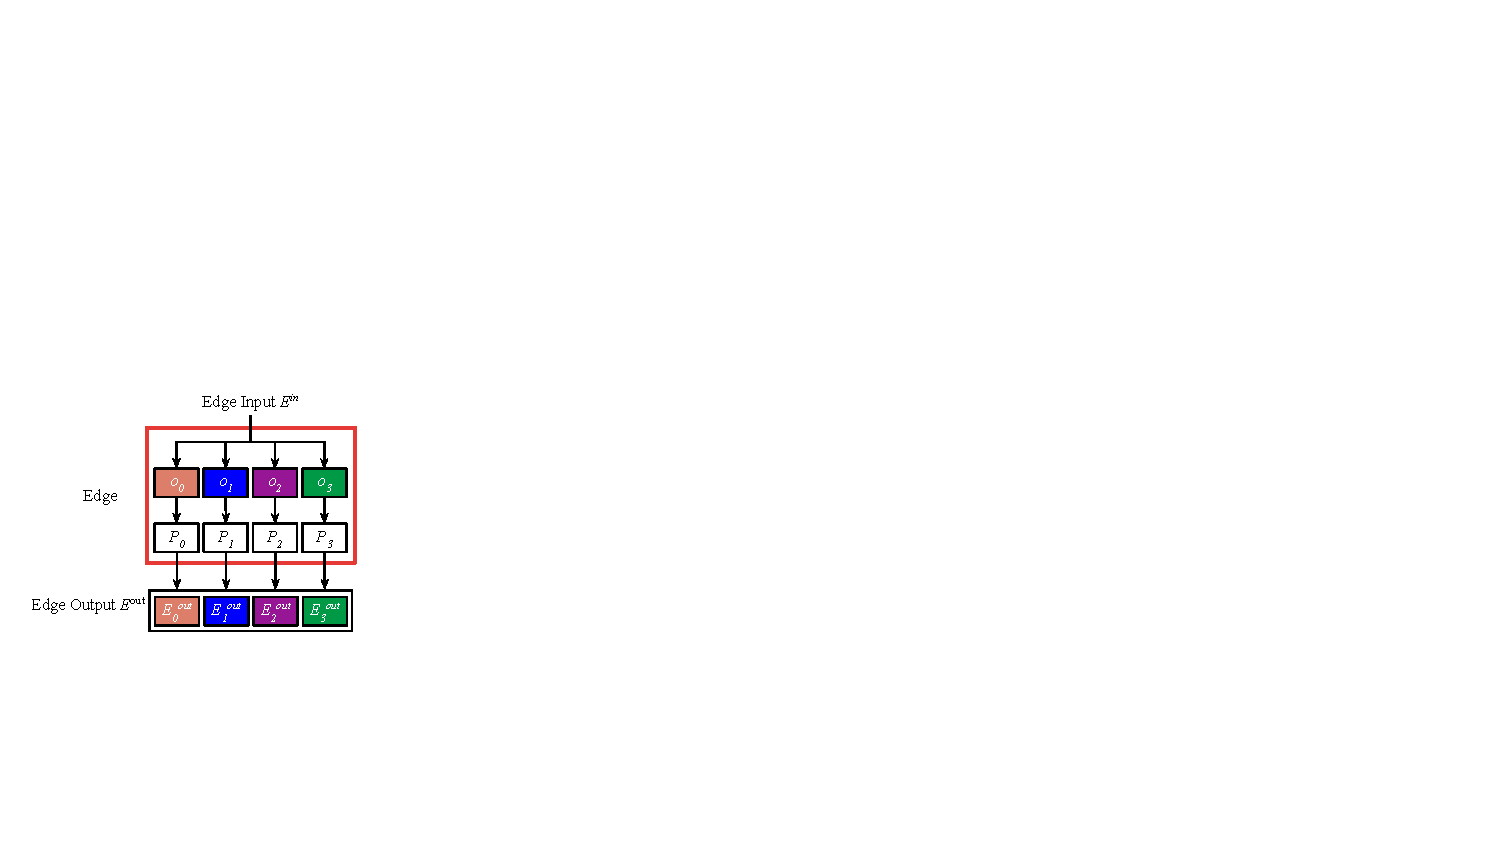
\includegraphics[width=.6\textwidth]{edge}
	\caption[Bonsai edge where $|\mathcal{O}|=4$]{Bonsai edge where $|\mathcal{O}|=4$.}
	\label{fig:bonsai_edge}
\end{figure}
\vspace{-1cm}
\newpage
\section{Nodes} \label{sect:bonsai_appendix_nodes}
Nodes (Figure~\ref{fig:bonsai_node}) concatenate the output lists of each inbound node via summation and batch normalization, and then pass this
concatenation on as the node output.
\begin{figure}[ht]
	\centering
	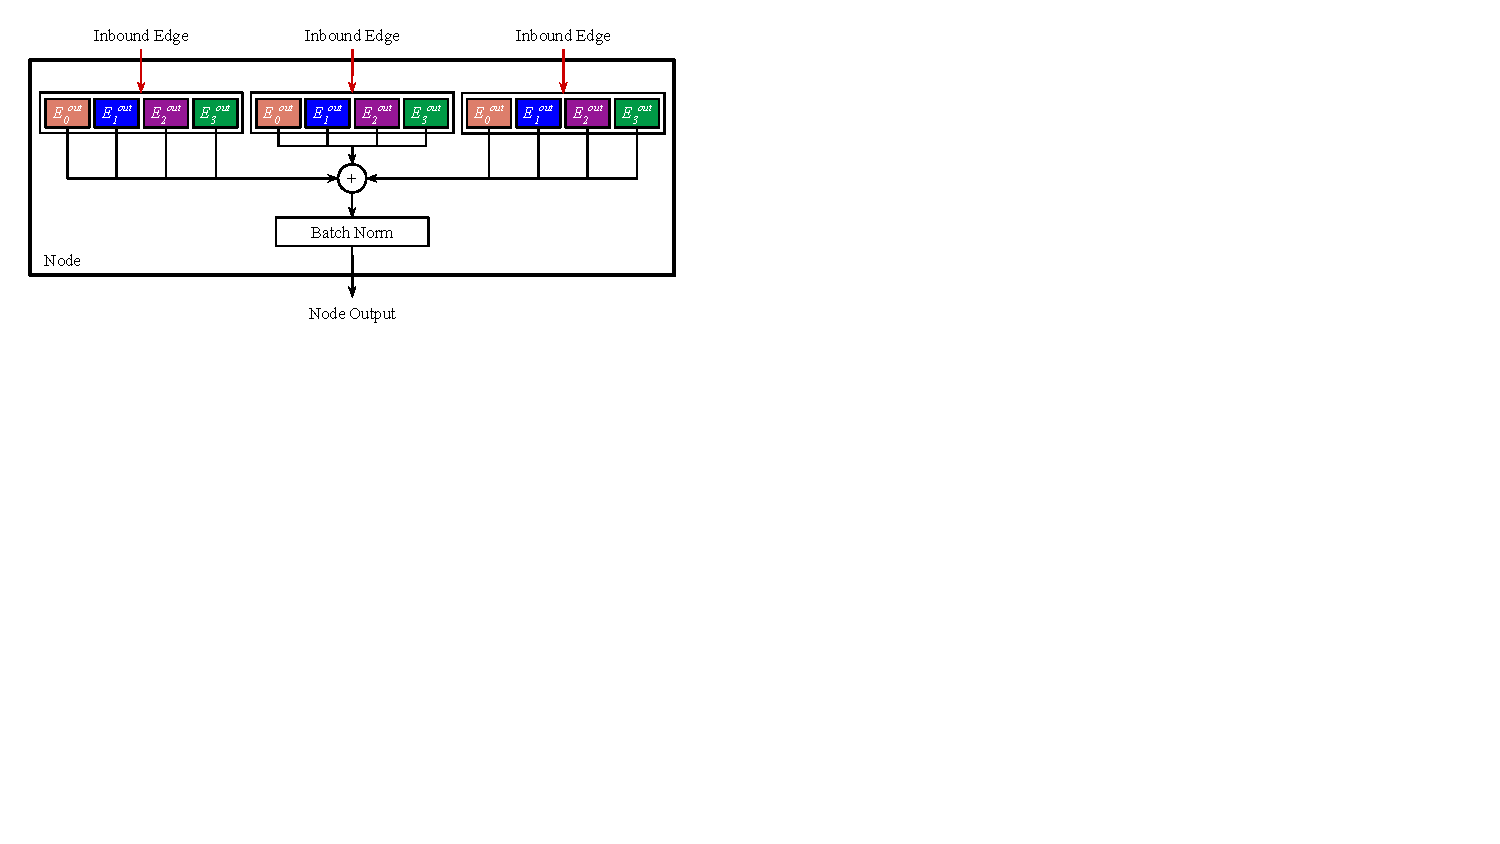
\includegraphics[width=.9\textwidth]{node}
	\caption[Bonsai node with three inbound Bonsai edges and $|\mathcal{O}|=4$]{Bonsai node with three inbound Bonsai edges and $|\mathcal{O}|=4$.}
	\label{fig:bonsai_node}
\end{figure}
\vspace*{-1cm}

\section{Cells} \label{sect:bonsai_appendix_cells}
Each cell receives the output of each antecedent cell and the original model input. These
inputs are processed through the cell input handler. The job of the input handler (Figure~\ref{fig:bonsai_ih})
is to scale the outputs of antecedent cells to be compatible with the operations in the cell and produce two outputs.
The first output is just the scaled output of the directly previous cell $C_{c-1}$. The second output is the pruned
sum of all antecedent cells [$C_{c-1}$, \dots, $C_{0}]$ as well as the original model input.

\begin{figure}[ht]
	\centering
	\hspace*{-1cm}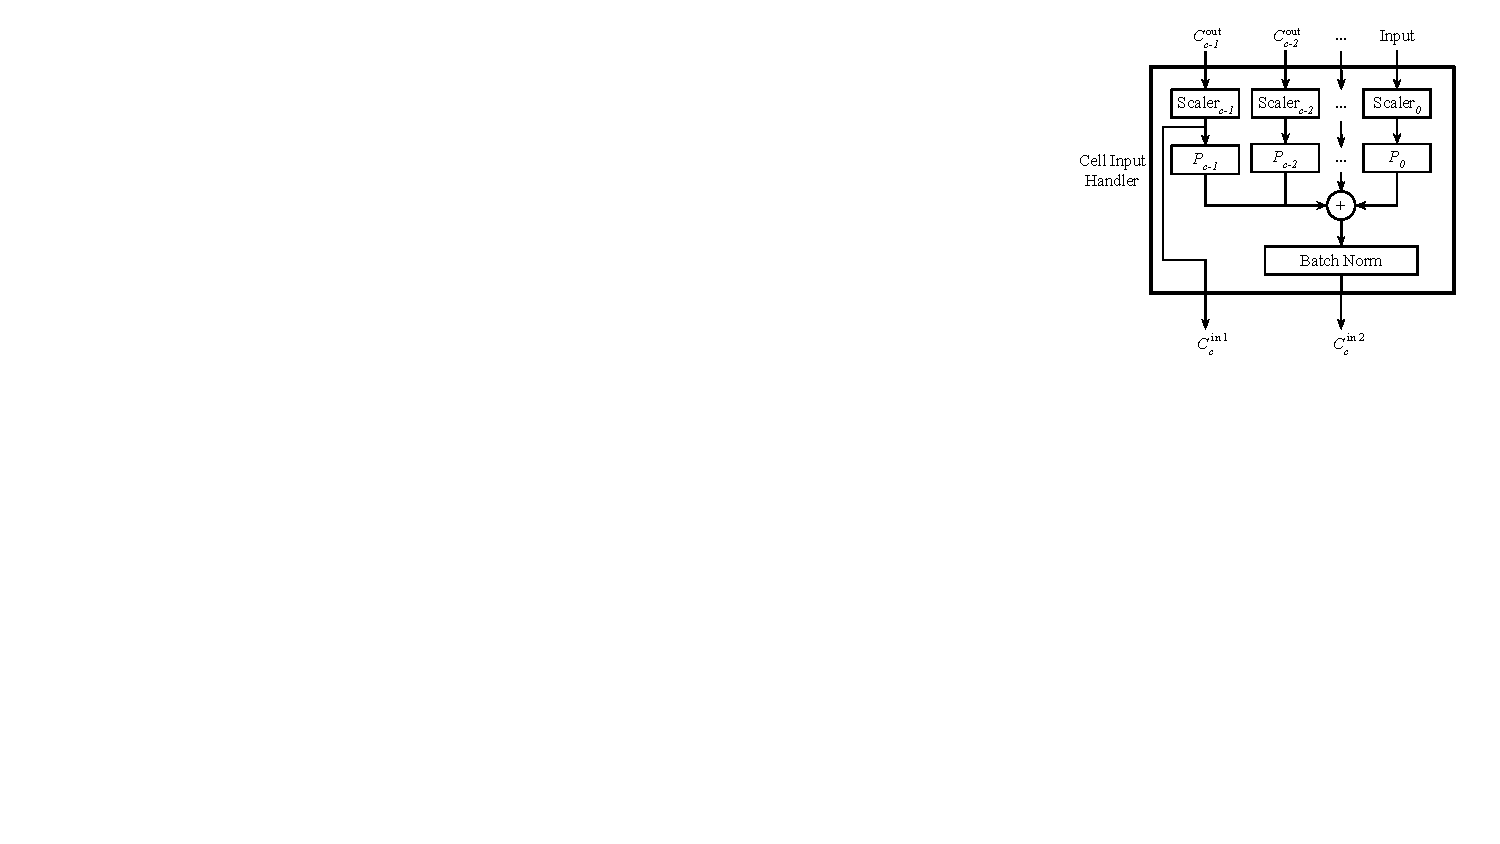
\includegraphics[width=.42\textwidth]{input_handler}
	\caption[The cell input handler]{The cell input handler.}
	\label{fig:bonsai_ih}
\end{figure}
These two outputs are
passed to the input nodes of the cell, called Node x and Node y. From here, each node $n$ is connected via Bonsai
edges to each node $[n+1, n+2, \dots, n+d]$ where $d$ is the edge depth of the model. This simply controls the width/depth
ratio of the model; a depth of 1 means every node is linearly connected in serial, while a depth equal to the number of
nodes means each node connects to every downstream node.
\begin{figure}[t!]
	\centering
	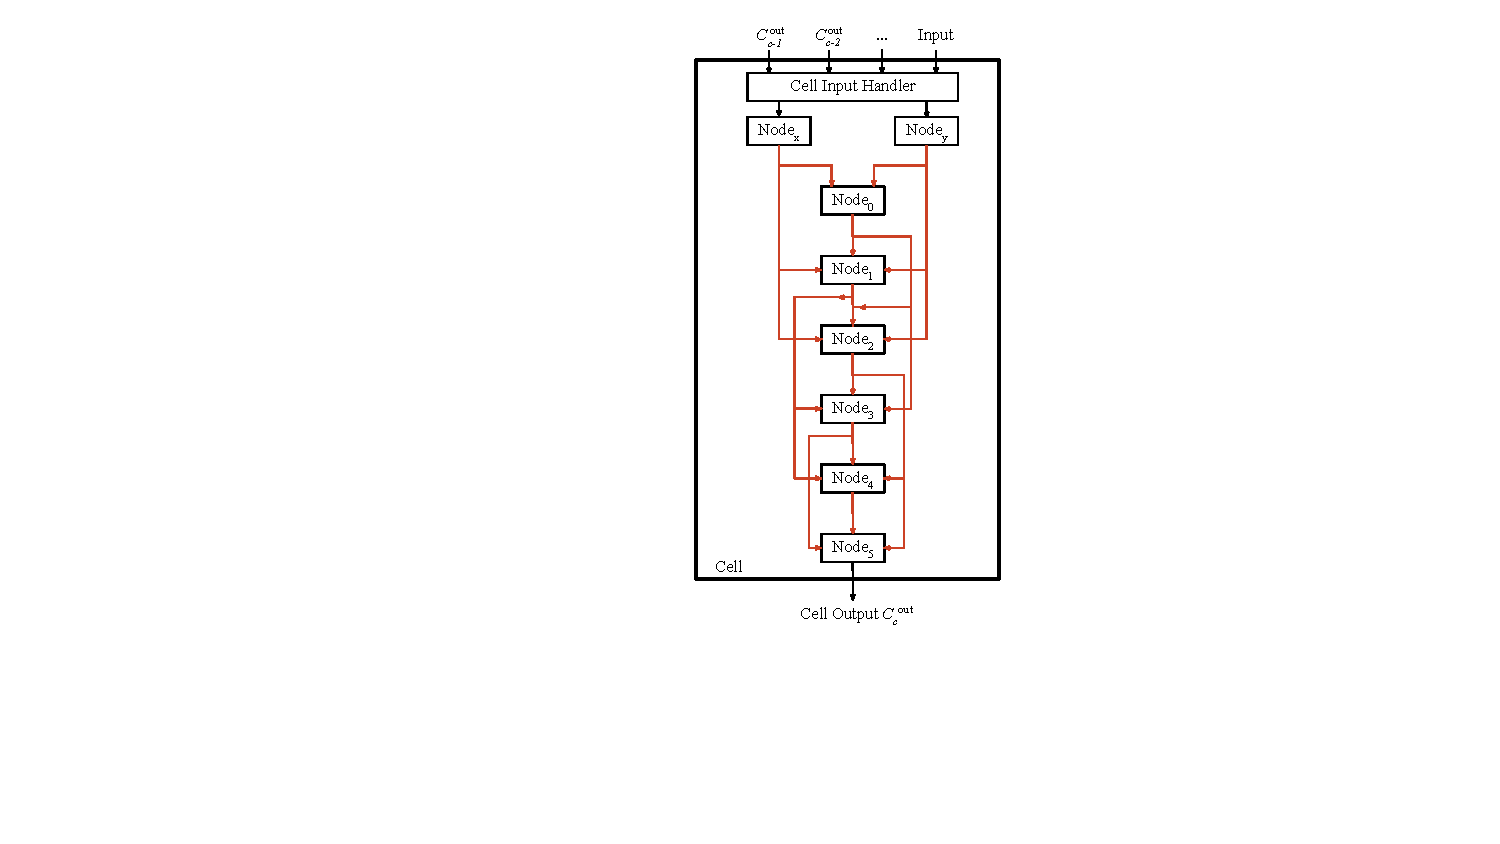
\includegraphics[width=.7\textwidth]{cell}
	\caption[Bonsai cell with six nodes and edge depth $d=3$]{Bonsai cell with six nodes and edge depth $d=3$. This depth means each node connects to each of the next
	three nodes.}
	\label{fig:bonsai_cell}
\end{figure}

\clearpage

\section{Models}
Bonsai models are comprised of stacked cells, where each cell receives the output of all previous cells and the original
model input. Cells are added in \textit{model sections} of $n$ cells as per the Bonsai search algorithm. The progression of a
model from one section to three sections, where each section consists of a single cell, is shown in Figure~\ref{fig:bonsai_growth}.
\begin{figure}[ht!]
\centering
\begin{subfigure}{.5\textwidth}
  \centering
  \vspace*{-.3cm}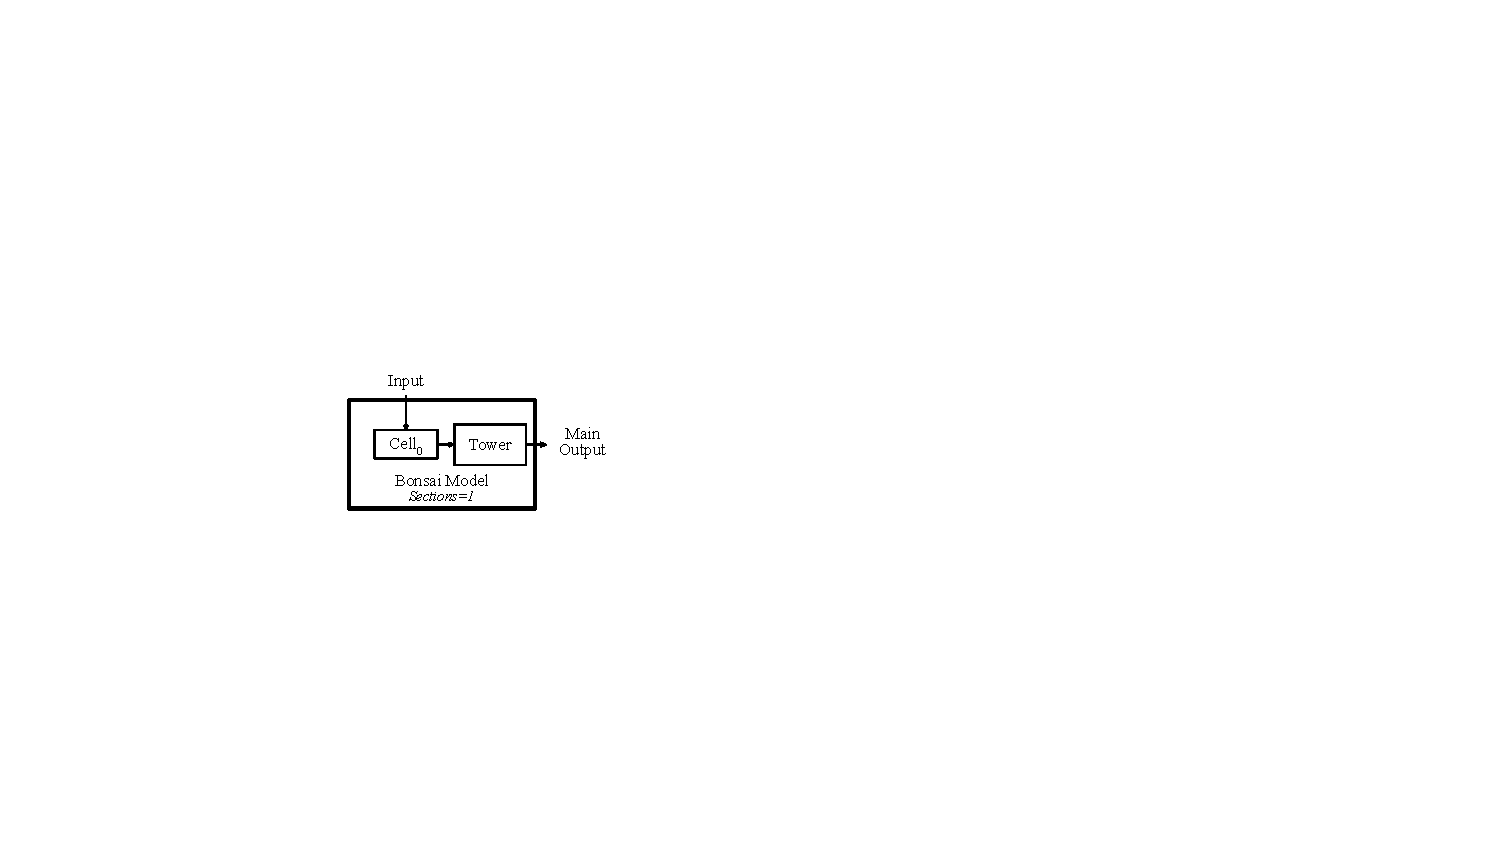
\includegraphics[width=.9\linewidth]{model1}
\end{subfigure}%
\begin{subfigure}{.5\textwidth}
  \centering
  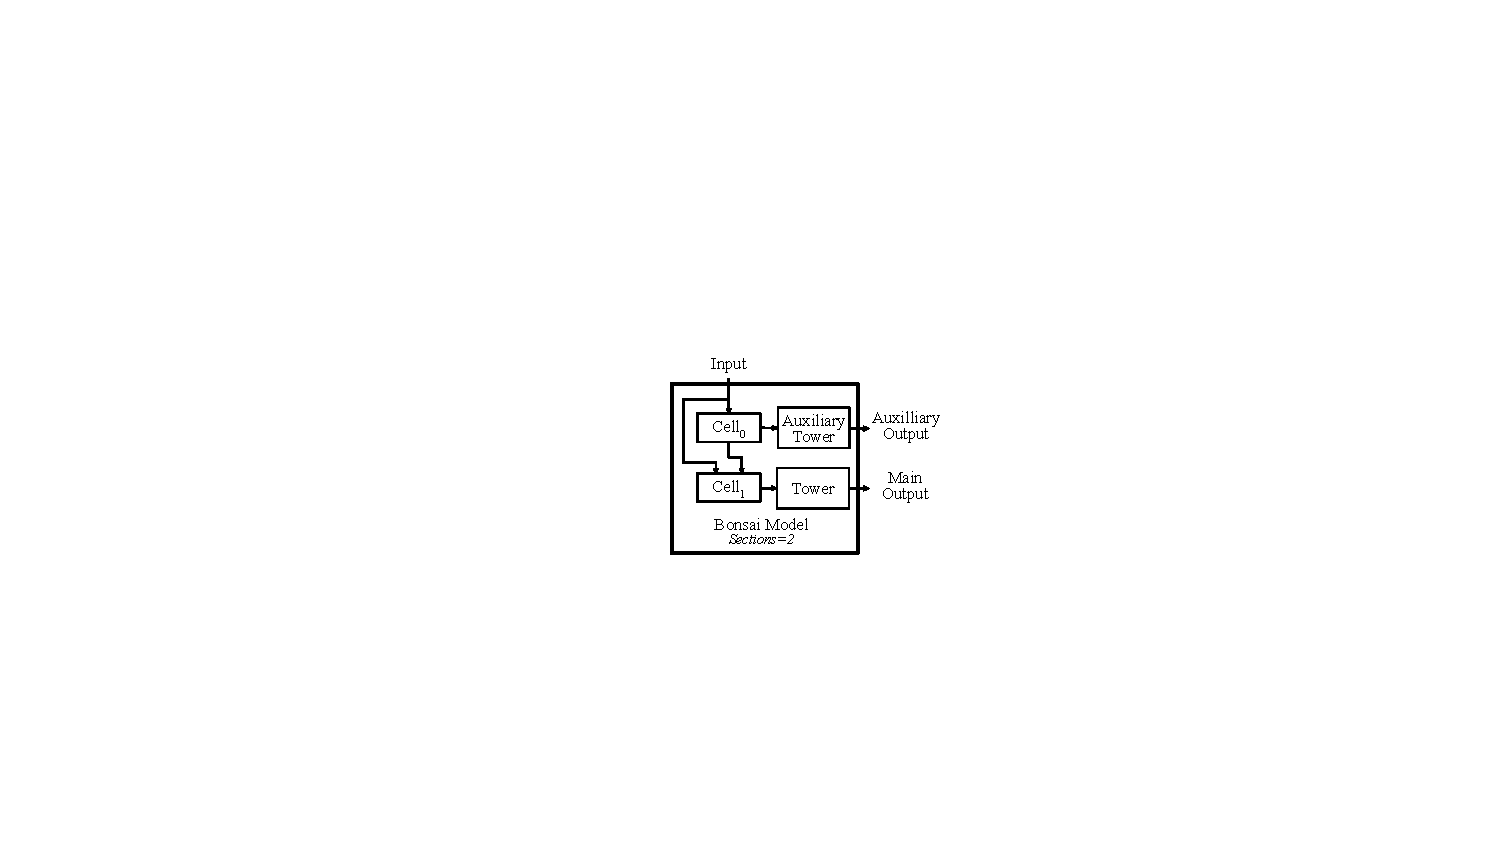
\includegraphics[width=.9\linewidth]{model2}
\end{subfigure}\\ \vspace{1em} \hrulefill \vspace{1em}
\begin{subfigure}{.5\textwidth}
  \centering
  \vspace*{-1.4cm}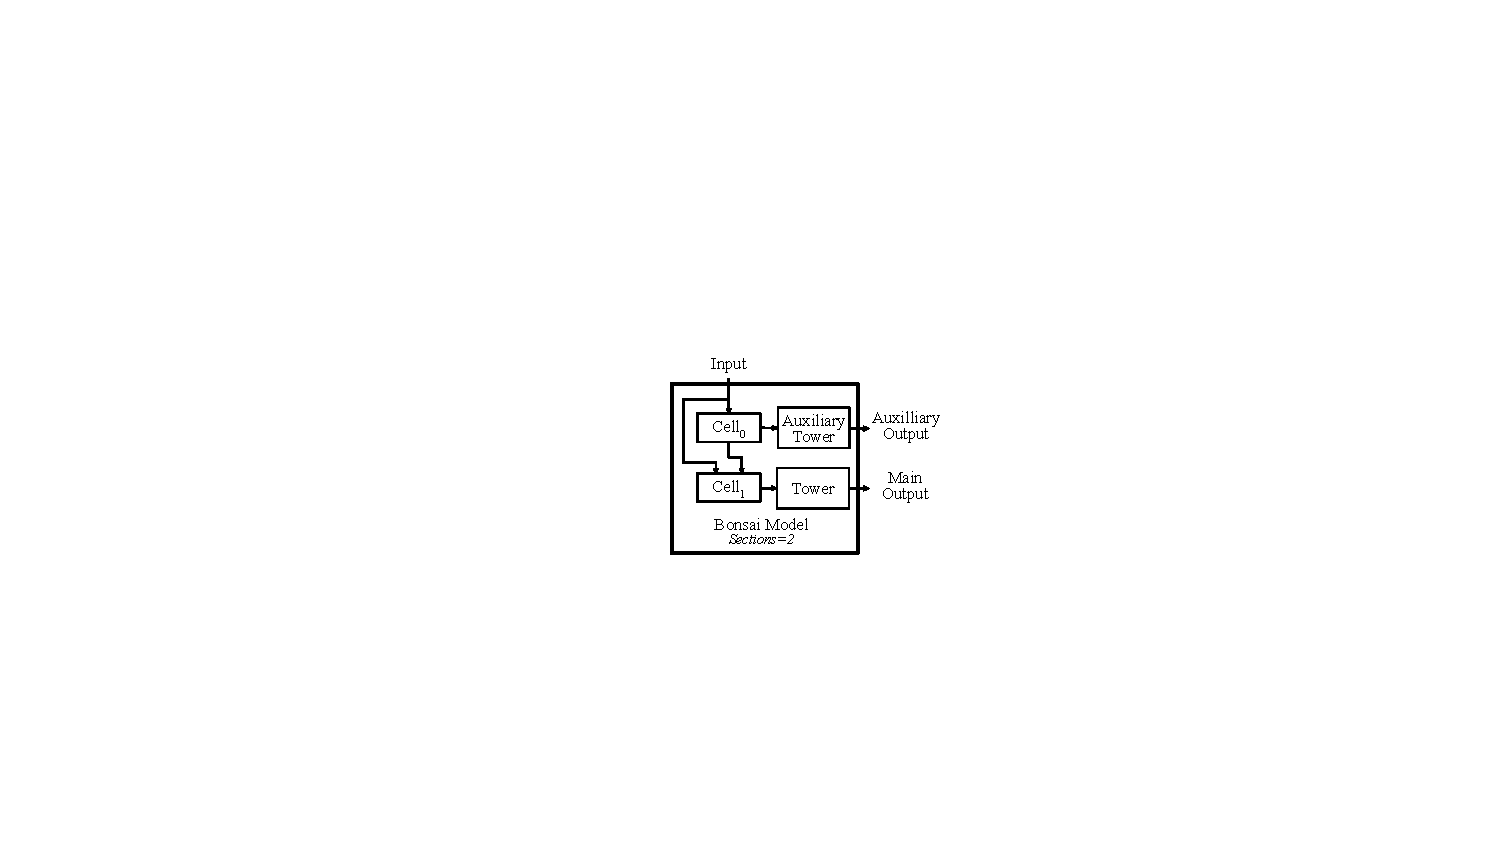
\includegraphics[width=.9\linewidth]{model2}
\end{subfigure}%
\begin{subfigure}{.5\textwidth}
  \centering
  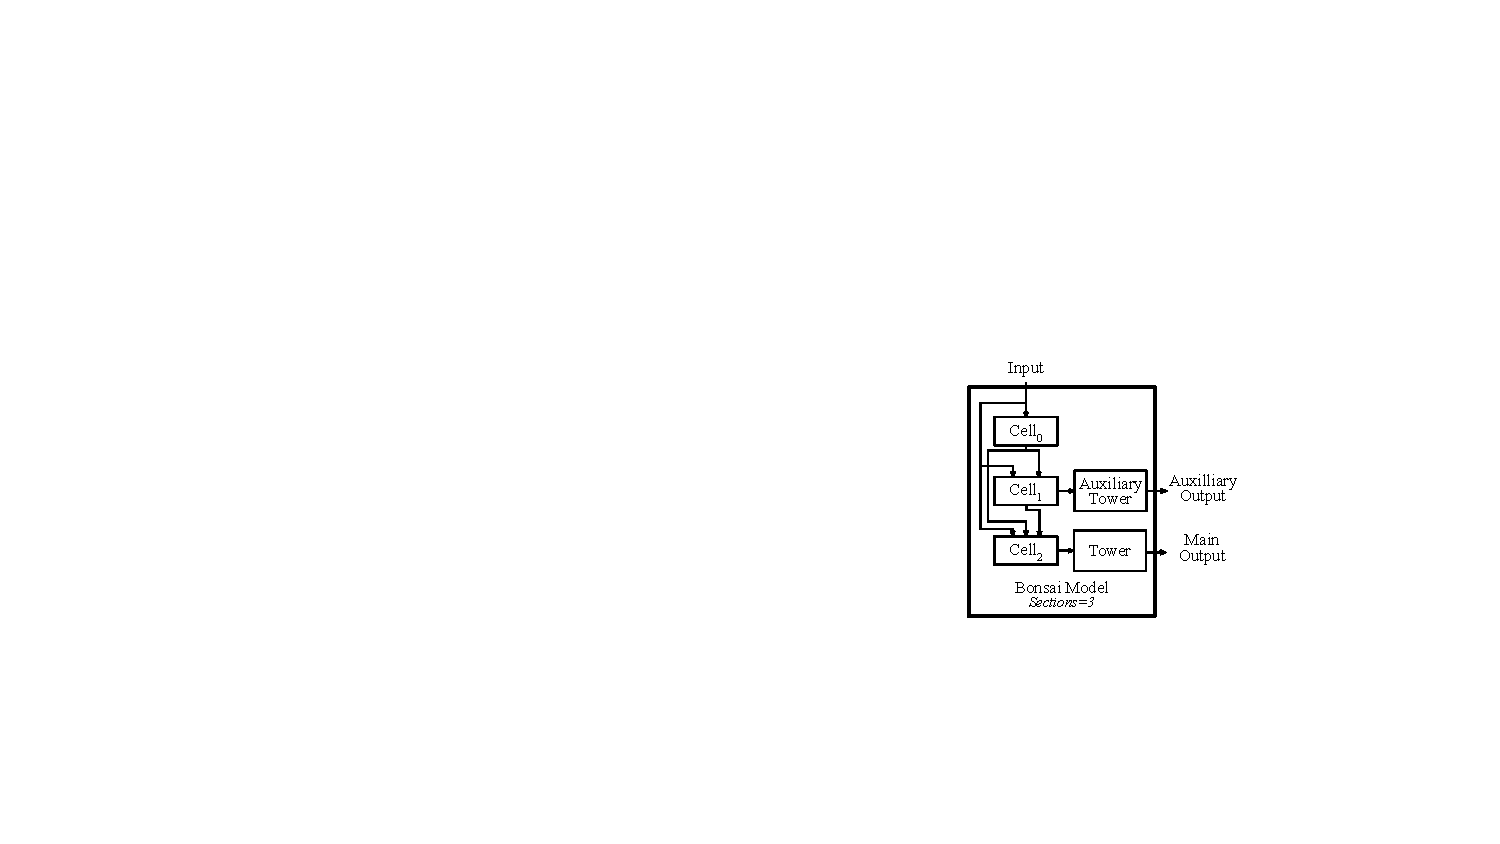
\includegraphics[width=.9\linewidth]{model3}
\end{subfigure}
\caption[The progression of a model from one through three sections]{The top row shows the progression of the model from one section to two sections. Note how the old output tower from
the previous section is converted into an auxilliary tower in the next. The bottom row shows the progression from two sections
to three sections.}
\label{fig:bonsai_growth}
\end{figure}

\clearpage

\section{Implementation Details} \label{sect:bonsai_implementation_details}
This section will discuss a few notes on how these algorithms are practically implemented within PyTorch. PyTorch was chosen
as the framework for this implementation specifically due to its \textit{dynamic computational graph}, that is, the graph
structure it uses to determine the forwards and backwards propagation of data and gradients through the model is dynamically
constructed each pass. This is in contrast to Tensorflow's static computational graph, which is determined once at initialization.
The dynamic graph allows the network connectivity to be modified in-place with ease during model training, a fundamental
necessity for pruning and deadheading.

\subsection{Working with Dynamic Parameter Counts}
An unforeseen snag of the Bonsai algorithm is the need for the parameter count of the model to change over time. Deadheading
drops a number of parameters from the model, while the addition of model sections can often multiplicatively increase the
total number of model parameters. The PyTorch optimizer needs to keep track of which parameters need to be differentiated,
which have been deleted, and which have been added, otherwise the backpropagated changes will only take effect on the
initial parameter configuration of the model.

Ensuring that the optimizer is aware of the parameters removed by deadheading is relatively straightforward; each pruner
carries a \texttt{switch\_off} method that can be called during the deadheading process. If the pruner is deadheaded,
the \texttt{switch\_off} method marks the pruner's weight parameter's \texttt{require\_grad} flag to \texttt{False}, which
indicates to the Torch optimizer that this parameter need not be updated during backpropagation. Furthermore, if an operation
is deadheaded, it is excluded from the forwards calculation of the model. This removes the operation from the computation
graph, which means that the backwards pass that the optimizer performs through the graph never comes across the deadheaded
operation. In combination, setting the flag and removing the operation from the computation graph ensures that the optimizer
can skip the deadheaded operation, which speeds up the forwards-backwards passes of the model after each deadheading.

Tracking new parameters is slightly trickier. While one approach is to collect all the new parameters from an added section and
simply append it to the optimizer, those parameters would be adjusted according to the current learning rate. Since
BonsaiNet models are trained according to a cosine annealing learning rate, sections added at later stages of
training would then see their first training under a significantly lower learning rate then the earlier sections
began training with. The question is, is that a desired behavior? My view is that since these new parameters are arriving into
the model at a random initialization, each set of new parameters starts about roughly equally `far' from optimized. Therefore,
using the global, already annealed learning rate for a set of new parameters will mean they will learn more slowly
than the original model parameters were able to. Instead, each new set of parameters $P$ added to the model tracks the
epoch $T^{P}_{added}$ at which they were added to their model, and sets their annealing rate accordingly:
\begin{align}
	\eta_t = \eta_{min} + \frac{1}{2}(\eta_{max}-\eta_{min})\left(1+ \cos \left(\left(\frac{T_{curr}-T^P_{added}}{T_{max}-T^P_{added}}\right) \pi \right)\right), \label{eq:tracked_annealing}
\end{align}

\noindent where $T_{curr}$ is the current, global model training epoch and $T_{max}$ is the desired total epoch count.
Therefore at the final epoch $T_{max}$ each set of parameters will be trained with a learning rate of $\eta_{min}$,
regardless of when they were added to the model. In practice, most Bonsai models get to their full size within a few dozen epochs,
so the epoch and thus annealing schedule difference between the original and final parameters is relatively minimal.
However, under certain configurations like the small cell case (see Section~\ref{sect:small_cell_introduction}) the model spends
quite a while pruning to accommodate for large sections, separating the original and final sections by over 100 epochs.
In this case the learning rate difference between the two is significantly more noticeable, and it would likely be
detrimental to train the new sections at the earlier sections' much lower learning rate. As such, the separate per-section
learning rate ensures that the training of each section is consistent throughout the model. However, further experiments would
be necessary to definitively confirm this.

\subsection{Pruner Implementation} \label{sect:pruner_implementation}
While the extensive usage of pruners through the supernet means there is a tremendous amount of architectural flexibility,
it does mean that the pruner calculation functions are called very frequently and as such need to be made as efficient as possible. To optimize the pruner function requires
creating gradient-safe tensor versions of equations~\ref{eq:gate} and~\ref{eq:saw} with the minimum number of function calls.
\textit{Gradient-safe} refers to ensuring that the gradient of the proposed tensor operation has the expected gradient
throughout the reasonable working range of the operation, and its output and gradient are always valid (finite and non-null).
This is crucial because an invalid output or gradient from a gradient-unsafe operation will cause every subsequent operation
in the network to produce invalid values, which then spread to the rest of the network in backpropagation.
This exemplifies the danger of gradient-unsafe operations, as a single invalid output or gradient will rapidly corrupt
an entire model.

Through experimenting with a variety of gate implementations, the following was chosen as having the minimum
number of underlying CUDA function calls and fastest execution time while remaining gradient safe:
\begin{align}
	G(w) &=  \texttt{boolean}(w > 0)
\end{align}
Since Torch computes gradients discretely, the computed gradient for all values of $w$ is uniformly 0;
it is impossible to sample a point that actually lies on the $w=0$ discontinuity of this particular function.

The next focus is the saw implementation. This needs to oscillate imperceptibly around 0 with a constant gradient of 1,
while remaining strictly greater than 0. This second criterion is important to make sure that the sign of the incoming tensor
is never flipped, such as to ensure the pruner is as transparent as possible. One possible implementation mirrors the equation
given in the original Differentiable Pruner paper~\citep{kim2019v1}:
\begin{align}
	S(w) &= \frac{M w - \lfloor M w \rfloor}{M} \label{eq:rawsaw}
\end{align}

This ``raw'' implementation is gradient-safe and performs mathematically correctly. However, it consists of four discrete operations
(the multiplication of $M$ by $w$, the floor operation, the subtraction, and the final division), which entails four total
tensor initializations to store the intermediate calculations of the operation as well as a high number of CUDA function calls.
As previously stated, the saw is in the absolute innermost loop of the model execution, and thus is a crucial area for optimization.
As such, the following optimized implementation was designed:
\begin{align}
	S(w) &= w\Mod{\frac{1}{M}} \label{eq:optsaw}
\end{align}

This is mathematically identical to the original raw implementation, but makes use of the in-built CUDA function for computing
moduli called \texttt{remainder}. The theoretical advantage here is that \texttt{remainder} is CUDA-native, meaning its forward
and backward calculation are already optimized on a compiler level. The function only involves a single CUDA operation,
meaning there is only a single new tensor that needs to be initialized which should save some VRAM space compared to the
previous implementation. Additionally, since $\frac{1}{M}$ is constant throughout the lifespan of the pruner it
can be precomputed at initialization, further reducing the runtime. Table~\ref{tab:saw_implementations}
compares the performance of the two implementations:

\begin{table}[h]
\begin{center}
\begin{tabular}{c|c|c|c|c}
& & \multicolumn{2}{c|}{Runtime per 100 calls, ms} &  \\
Saw & CUDA Functions & Forward & Forward+Backward & VRAM\\
		  \hline
Raw		& 2 mul, 2 floor, 1 sub, 4 tensor init & 13.3 & 129.1 & 1200 Kb\\
Optimized     & 1 remainder, 1 tensor init & 2.8 & 18.3 & 100 Kb\\
\end{tabular}
\end{center}
\caption[Comparison of raw and optimized saw implementations]{Comparison of raw and optimized saw implementations. CUDA function calls and
runtimes determined via the PyTorch profiler, while VRAM allocations were measured in a process similar to that of Bonsai operation
sizing detailed in Algorithm~\ref{alg:revised_operation_sizing}.}
\label{tab:saw_implementations}
\end{table}

Checking runtime across both forward and forward-backward use cases is very important, specifically to check that
any performance advantage is present across both use cases. While only checking the forward pass is
the easier test to perform, the forward-backward use case is much more representative of the real-world application of any
particular operation. This is due to heavy reliance on the backwards operation during SGD training, and the cost
of the backwards operation being entirely independent of the cost of the forward operation. There are many times in the development
of this optimizations wherein two candidate functions were compared, and while one was faster than the other in the forward use case,
its backward operation was orders of magnitude slower and thus completely cancelled out the forward advantage.
Operations like tensor indexing and the \texttt{sign} function are two such examples of these deceptive functions.
The remainder operation thankfully does not exhibit such deceptiveness, with results showing that the optimized saw runs
around seven times faster than the raw saw in both use-cases. Furthermore, the need to initialize only a single tensor for
the optimized saw results in a $12\times$ VRAM savings as compared to the raw saw.

\section{Random Search Algorithms}
\begin{algorithm}[ht!]
\SetAlgoLined
Given some BonsaiNet model $M^{[0,1,\dots,n]}_{[c_0,c_1,\dots, c_n]}$ to emulate\;
Initialize an empty model R\;
\BlankLine
\For{i in $[0, n-1$]}{
	Fill model section $R^i$ with operations at random until it reaches compression $c_i$\;
	Add the model section to the random model: $R = R + R^i_{c_i}$\;
}
Add the final section uncompressed: $R = R + R^n_{1}$\;
Train the resultant model $R^{[0,1,\dots,n]}_{[c_0,c_1,\dots,1]}$ \textbf{with pruning} and according to the same hyperparameters used for $M$\;
\caption{Random 1}
\label{alg:bonsai_r1}
\end{algorithm}

\begin{algorithm}[ht]
\SetAlgoLined
Given some BonsaiNet model $M^{[0,1,\dots,{n}]}_{[c_0,c_1,\dots,c_{n}]}$ to emulate\;
Initialize an empty model R\;
\BlankLine
\For{i in $[0, n$]}{
	Fill model section $R^i$ with operations at random until it reaches compression $c_i$\;
	Add the model section to the random model: $R = R + R^i_{c_i}$\;
}
Train the resultant model $R^{[0,1,\dots,n]}_{[c_0,c_1,\dots,1]}$ \textbf{without pruning} and according to the same hyperparameters used for $M$\;
\caption{Random 2}
\label{alg:bonsai_r2}
\end{algorithm}
